\documentclass[11pt]{article}
\usepackage{textcomp}
\usepackage{fontenc}

\usepackage{graphicx}
\usepackage{caption}
\usepackage{sidecap}
\usepackage{enumitem}
\usepackage{multicol}
\usepackage{gensymb}
\usepackage{placeins}
\setlength{\parskip}{3 mm}

\graphicspath{{images/}}	% Root directory of the figures

\title{Photoperiod and temperature interactively drive spring phenology in multiple species}

\renewcommand*{\familydefault}{\sfdefault}



\begin{document}

\maketitle
\section{Abstract}

Woody plant spring phenology drives global carbon cycles and local ecosystem properties. Understanding the sensitivity of forest plants at the species level to abiotic drivers of plant phenology is thus critical for developing predictions of community and ecosystem-level properties. While observational studies of long-term trends are essential for understanding how climate affects timing of phenological events, experimental manipulations can disentangle otherwise covarying environmental factors and directly assess species- and individual-level responses to climate change factors.
Here we present results from a chilling x photoperiod x warming experiment with dormant clippings taken from two different latitudes (42.5 N and 46 N) to address how these interactive effects drive spring leafout phenology across 28 North American woody species. We found photoperiod sensitivity is common in northeastern woody plants and phenological sensitivity to photoperiod and temperature appears largely coordinated across species (i.e., species highly sensitive to temperature were also highly sensitive to photoperiod). Effects of chilling at 1.5 C were less pronounced than effects at 4 C. Overall, however, initial analyses suggest a small role for site (latitude) and chilling in affecting spring phenology. Shrub and small tree species were more sensitive to warming and thus may be more opportunistic with novel climate conditions. In contrast, larger tree species, being less sensitive to temperature cues, may be challenged.

\section{Introduction}


Woody plant spring phenology drives global carbon cycles and local ecosystem properties. Understanding the sensitivity of forest plants at the species level to abiotic drivers of plant phenology is thus critical for developing predictions of community and ecosystem-level properties. 

While observational studies of long-term trends are essential for understanding how climate affects timing of phenological events, experimental manipulations can disentangle otherwise covarying environmental factors and directly assess species- and individual-level responses to climate change factors. 

Here we ask the following questions:
\begin{itemize}
\item{For a suite of northeastern woody plants, what is the role of photoperiod versus temperature in determining timing of budburst, leaf-out, and flowering? Are species limited by photoperiod requirements in their response to warming temperatures?}
\item{To what extent do winter chilling requirements act as additional conservative strategy to avoid damage from early spring freezing?}
\item{Do populations at northern sites, with more severe winters and shorter winter daylength, exhibit more conservative phenological strategies?}
\end{itemize}


Dormancy notes
Conflicting role of photoperiod in tree phenology 
Depending on phenological stage, species and location (Heide 1993; Kramer 1994; Falusi and Calamassi 1996). 
From Chine et al. 2013 book chapter:
long photoperiod enhances cell growth, compensating for a lack of chilling during the endodormancy phase (Wareing 1953; Heide 1993b; Myking and Heide 1995; Caffarra et al. 2011a).

Hanninen divided into sequental and parallel, Chuine 2000 unified.

A literature review found 90 studies which investigated effects of photoperiod, temperature, or their interaction on the timing of bud burst or flowering for woody or semi-woody plants.  No study varied chilling period, photoperiod, and temperature simultaneously across multiple species at multiple sites. Of those studies, eight simultaneously manipulated photoperiod and temperature. 




\section{Materials and Methods}

To test effects of temperature and photoperiod
Woody plant cuttings were made in January 2015 for 28 species which occurred in both Harvard Forest (HF, 42.5\degree N, 72.2\degree W) and the Station de Biologie des Laurentides in St-Hippolyte, Quebec (SH, 45.9\degree N, 74.0\degree W). Cuttings were grown in growth chambers at the Arnold Arboretum in Boston, MA, in distilled water, with water changed every 7-10 days. Cuttings of an individual tree were exposed to each of 12 experimental treatments in a fully-factorial design: 2 temperature (20\degree C / 10\degree C warm vs. 15\degree C / 5\degree C cool) x 2 photoperiod (12 vs. 8 h) x 3 chilling (zero,  33 d at 4\degree C, 33 d at 1.5\degree C) treatments. 

With 6 replicates of these species across 6 experimental treatments being monitored at 5-7 day intervals for over 3 months, we made over 17,500 individual phenological observations following a modified BBCH scale.


\section{Results}

Temperature and photoperiod individually and interactively determined timing of leaf-out, with strongest effects of temperature in short-day conditions. We found increasing photoperiod significantly reduced time to phenological responses overall and for individual species, across sites of origin. 

For the 28 species studied, sensitivity to temperature and photoperiod cues for leaf-out times varied substantially, and surprisingly co-varied overall. The coordinated response to warming temperatures and longer photoperiod was consistent with overall pace of phenological events; earlier-leafing out species (namely the shrubs \emph{Spiraea alba}, \emph{Viburnum cassanoides}, and \emph{Vaccinium myrtilloides}) exhibited relatively limited advances to either warming or longer days, while later leafing-out species showed ability to advance their phenology by in response to both warming and longer days. Thus, no trade-off was observed between photoperiod-cued and temperature-cued species, but rather species exhibit coordinated responses to both environmental factors (Fig. 1).

Figure 1. Coordinated responses of 28 woody plant species to photoperiod and temperature cues for leafout. Size of circle reflect average leafout day across treatments, across sites of origin.

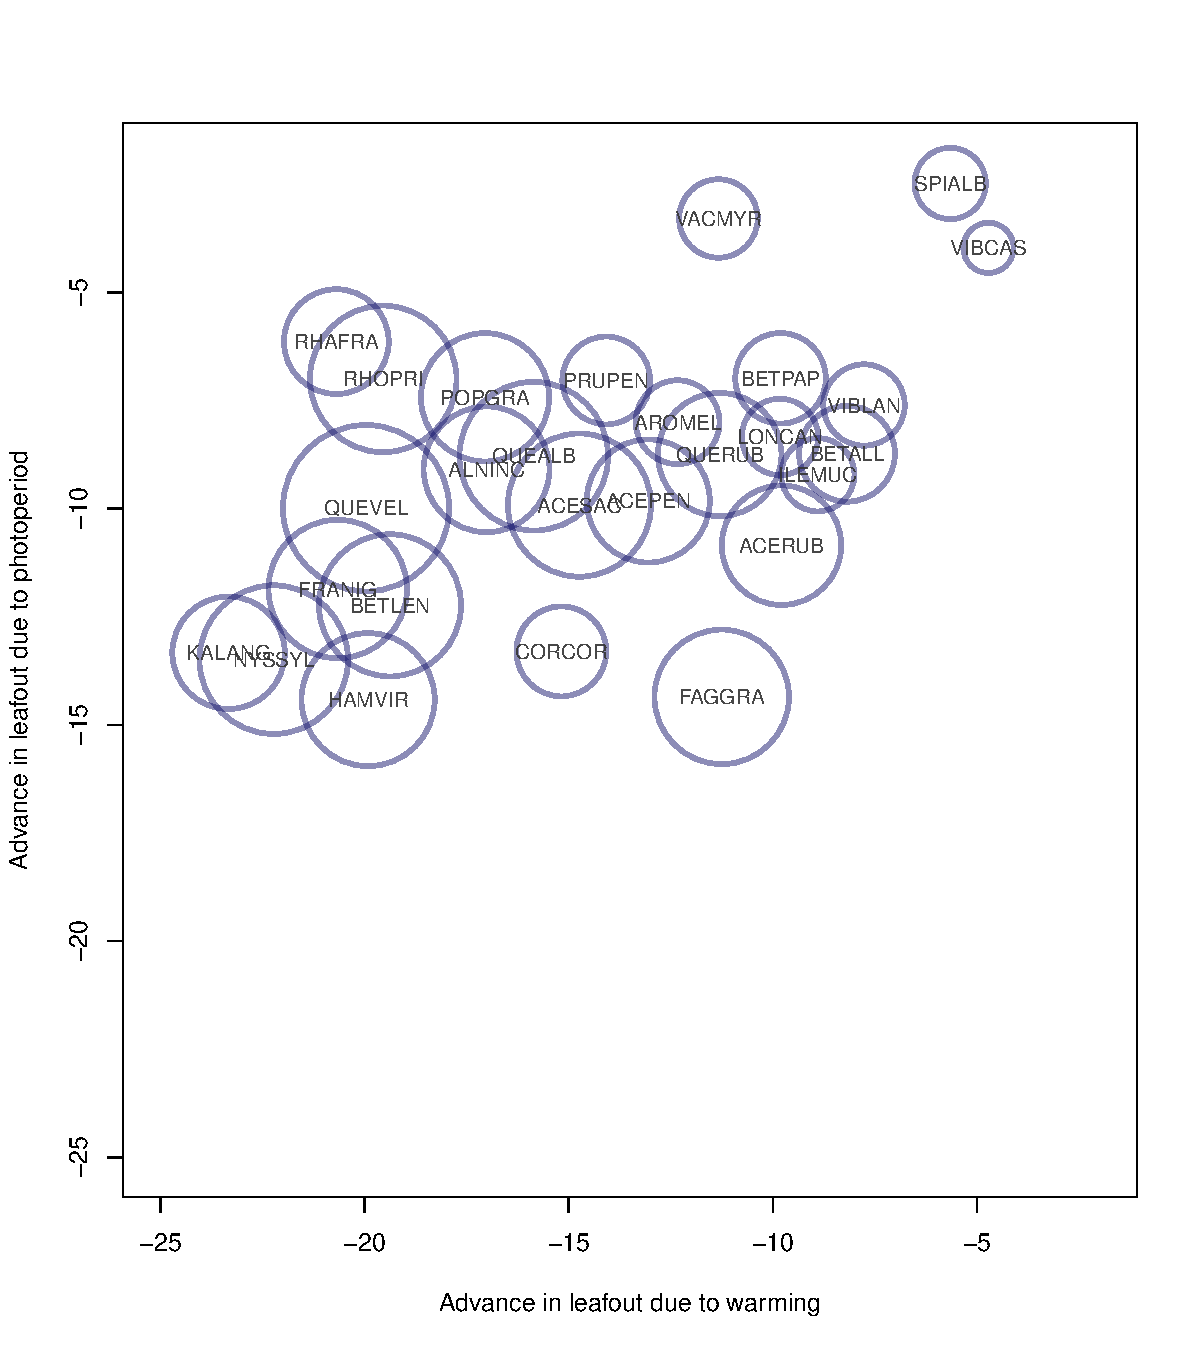
\includegraphics[scale=0.5]{Advplot}

While both photoperiod and temperature cues were important for driving woody plant phenology, responses to chilling were also substantial. Budburst day was accelerated most by the chilling treatments. Tables 1 and 2 summarizes mixed-effects model analysis of day of budburst and leaf-out, with negative values indicate earlier day of experiment for each event. Overall the 5\degree C experimental warming resulted in 2.2 days earlier budburst and 5.5 days earlier leafout. Such advance was delayed by the severe chilling treatment. Latitude of origin overall had little direct effect on budburst or leaf-out, but populations from the northern site tended to exhibit more rapid leaf-out under the severe chilling treatment.

% from Pheno budburst analyses.R, using memisc and xtable

Warming, photoperiod, and chilling individually and interactively acted to drive budburst and leafout earlier across species. The strength of the acceleration in budburst due to both warming and photoperiod were similar, but the acceleration of leafout due to warming exceeded that of photoperiod. Surprisingly, site of origin exerted no effect on either budburst or leafout across species. 

Table 1. Summary of mixed effect model of budburst day by species

\FloatBarrier
\begin{table}[ht]
\centering
\begin{tabular}{rrrrrrr}
  \hline
 & est & se & stat & p & lwr & upr \\ 
  \hline
(Intercept) & 25.90 & 1.75 & 14.76 & 0.00 & 22.46 & 29.34 \\ 
  warmn & -2.20 & 0.43 & -5.16 & 0.00 & -3.03 & -1.36 \\ 
  photon & -2.50 & 0.39 & -6.34 & 0.00 & -3.27 & -1.73 \\ 
  siteSH & -0.41 & 0.43 & -0.96 & 0.34 & -1.24 & 0.43 \\ 
  chilln & -3.99 & 0.33 & -11.93 & 0.00 & -4.65 & -3.34 \\ 
  warmn:photon & -0.20 & 0.28 & -0.73 & 0.46 & -0.75 & 0.34 \\ 
  warmn:siteSH & -0.49 & 0.41 & -1.18 & 0.24 & -1.29 & 0.32 \\ 
  photon:siteSH & 0.06 & 0.41 & 0.14 & 0.89 & -0.75 & 0.87 \\ 
  warmn:chilln & 2.16 & 0.30 & 7.16 & 0.00 & 1.57 & 2.75 \\ 
  photon:chilln & -0.11 & 0.31 & -0.34 & 0.73 & -0.71 & 0.50 \\ 
  siteSH:chilln & -0.52 & 0.44 & -1.18 & 0.24 & -1.37 & 0.34 \\ 
  warmn:photon:siteSH & -0.13 & 0.41 & -0.32 & 0.75 & -0.93 & 0.67 \\ 
  warmn:photon:chilln & -0.59 & 0.29 & -2.02 & 0.04 & -1.17 & -0.02 \\ 
  warmn:siteSH:chilln & -0.31 & 0.42 & -0.74 & 0.46 & -1.14 & 0.51 \\ 
  photon:siteSH:chilln & 0.06 & 0.42 & 0.15 & 0.88 & -0.77 & 0.89 \\ 
  warmn:photon:siteSH:chilln & 0.06 & 0.42 & 0.14 & 0.89 & -0.77 & 0.88 \\ 
           Var(\~{}1$|$sp) & 60.41 &  &  &  &  &  \\ 
       Var(\~{}warmn$|$sp) & 2.72 &  &  &  &  &  \\ 
     Cov(\~{}1:warmn$|$sp) & -12.82 &  &  &  &  &  \\ 
         Var(\~{}1$|$sp.1) & 22.57 &  &  &  &  &  \\ 
    Var(\~{}photon$|$sp.1) & 1.88 &  &  &  &  &  \\ 
  Cov(\~{}1:photon$|$sp.1) & -6.52 &  &  &  &  &  \\ 
        Var(residual) & 68.42 &  &  &  &  &  \\ 
   \hline
\end{tabular}
\end{table}
\FloatBarrier

%%%%%%%%%%% Figures for these tables
Figure 2. Summary of mixed effect model of days to budburst as predicted by temperature, photoperiod, chilling, site, and species.

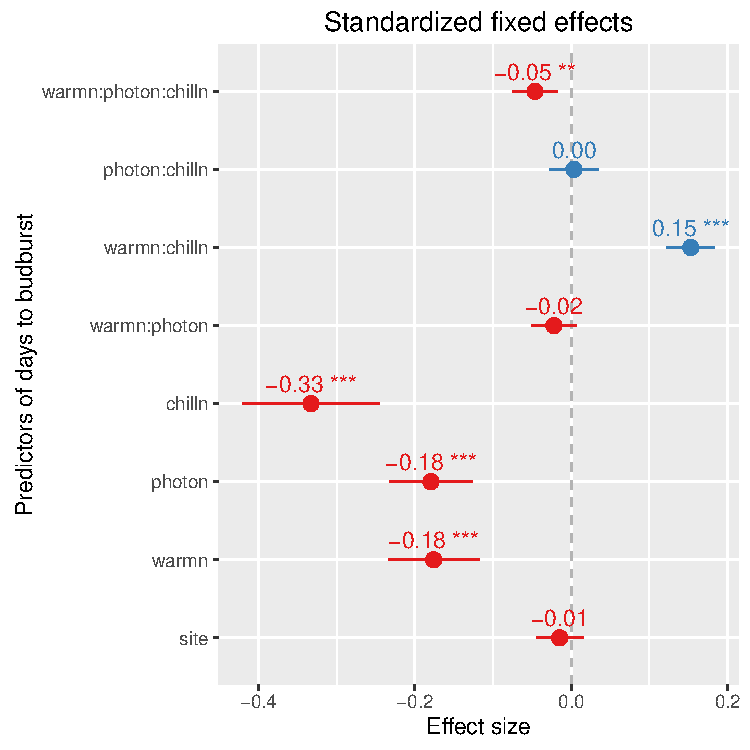
\includegraphics[scale=0.5]{lmerDBB}


Table 2. Summary of mixed effect model of leafout day by species.
\FloatBarrier
\begin{table}[H]
\centering
\begin{tabular}{rrrrrrr}
  \hline
 & est & se & stat & p & lwr & upr \\ 
  \hline
(Intercept) & 38.24 & 1.99 & 19.22 & 0.00 & 34.34 & 42.14 \\ 
  warmn & -5.50 & 0.76 & -7.21 & 0.00 & -7.00 & -4.01 \\ 
  photon & -3.78 & 0.70 & -5.38 & 0.00 & -5.16 & -2.40 \\ 
  site & 0.29 & 0.46 & 0.63 & 0.53 & -0.61 & 1.18 \\ 
  chilln & -3.83 & 0.76 & -5.07 & 0.00 & -5.32 & -2.35 \\ 
  warmn:photon & 0.98 & 0.68 & 1.45 & 0.15 & -0.34 & 2.30 \\ 
  warmn:site & -0.44 & 0.44 & -1.00 & 0.32 & -1.30 & 0.42 \\ 
  photon:site & -0.46 & 0.44 & -1.04 & 0.30 & -1.32 & 0.41 \\ 
  warmn:chilln & 3.72 & 0.71 & 5.23 & 0.00 & 2.33 & 5.12 \\ 
  photon:chilln & 1.21 & 0.71 & 1.69 & 0.09 & -0.19 & 2.61 \\ 
  site:chilln & -0.43 & 0.46 & -0.92 & 0.36 & -1.34 & 0.49 \\ 
  warmn:photon:site & -0.13 & 0.44 & -0.30 & 0.76 & -0.99 & 0.72 \\ 
  warmn:photon:chilln & -1.63 & 0.70 & -2.31 & 0.02 & -3.01 & -0.25 \\ 
  warmn:site:chilln & -0.75 & 0.45 & -1.66 & 0.10 & -1.63 & 0.13 \\ 
  photon:site:chilln & -0.45 & 0.45 & -1.01 & 0.31 & -1.34 & 0.43 \\ 
  warmn:photon:site:chilln & 0.40 & 0.45 & 0.89 & 0.37 & -0.48 & 1.28 \\ 
           Var(\~{}1$|$sp) & 80.60 &  &  &  &  &  \\ 
       Var(\~{}warmn$|$sp) & 3.40 &  &  &  &  &  \\ 
     Cov(\~{}1:warmn$|$sp) & -16.57 &  &  &  &  &  \\ 
         Var(\~{}1$|$sp.1) & 16.75 &  &  &  &  &  \\ 
    Var(\~{}photon$|$sp.1) & 0.95 &  &  &  &  &  \\ 
  Cov(\~{}1:photon$|$sp.1) & -3.99 &  &  &  &  &  \\ 
        Var(residual) & 78.07 &  &  &  &  &  \\ 
   \hline
\end{tabular}
\end{table}
\FloatBarrier
%%%%%%%%%%% Figures for this table
Figure 3. Summary of mixed effect model of days to leafout as predicted by temperature, photoperiod, chilling, site, and species.

\begin{center}
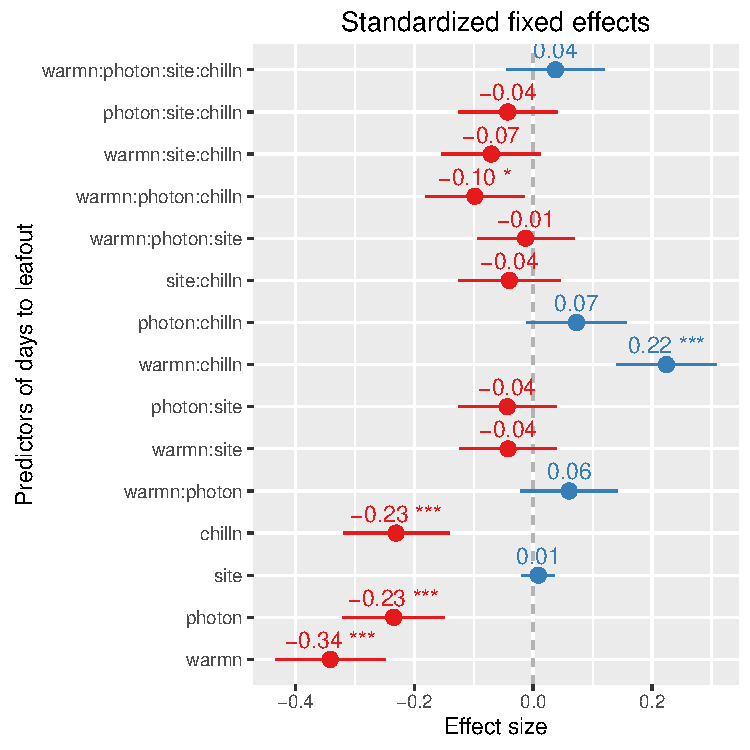
\includegraphics[scale=0.5]{lmerDLO}
\end{center}

\subsection*{Effect of chilling}
The cuttings were harvested in late January 2015, and thus experienced substantial chilling in the field. Using weather station data from the Harvard Forest site, chilling hours (below 7.2�C), Utah Model chill portions (hours below 7.2�C and between 0�C and 7.2�C) and Dynamic Model chill portions (Erez \& Fishman 1997) were calculated both for the natural chilling experienced by harvest and the chilling experienced in the 4�C and 1.5�C treatments. With both the Utah and Dynamic model, the more severe chilling treatment resulted in fewer calculated chilling portions.

Species varied widely in response to chilling treatments, with some exhibiting strong chilling requirements (\emph{Acer saccharum}, \emph{Fagus grandifolia}), while others exhibited little change in phenological advacement under experimentally manipulated chilling. Overall, leaf-out was advanced by 4.5 days under additional 30 d of vernalization at 4\degree C, and non-significantly delayed 0.67 days under additional 30 d of vernalization at 1.5\degree C.

Response of \emph{Fagus grandifolia} to increasingly strong vernalization varies by latitude of origin and by phenological stage; winter chilling reduced day to budburst (right) and leaf-out (left), but more strongly for individuals from the northern SH site.



\FloatBarrier
\begin{table}[ht]
\centering
\begin{tabular}{rlrrrr}
  \hline
 & Treatment & Days & Chilling\_Hours & Utah\_Model & Chill\_portions \\ 
  \hline
1 & Field chilling & 80.00 & 686.00 & 494.00 & 39.14 \\ 
  2 & 4.0� x 30 d & 119.00 & 1622.00 & 1430.00 & 66.96 \\ 
  3 & 1.5� x 30 d & 119.00 & 1622.00 & 1160.00 & 64.78 \\ 
   \hline
\end{tabular}
\end{table}
\FloatBarrier

While nearly all species showed advances in spring phenology in response to the experimental chilling treatment, as indicated by fewer days to phenological events for the 4�C and 1.5�C treatments, the majority of species (e.g. \emph{Populus grandidentata} showed delays in both budburst and leafout at the more severe chilling treatment. Of the species exposed to the additional chilling, only \emph{Fagus grandifolia} was consistently advanced by the more severe chilling (Fig. 4)

Figure 4. Frequency of days to budburst and leaf-out for two of the 28 species under the three chilling treatments, no additional chilling (0), additional 30 days at 4.0�C, or additional 30 days at 1.5�C.  

\begin{center}
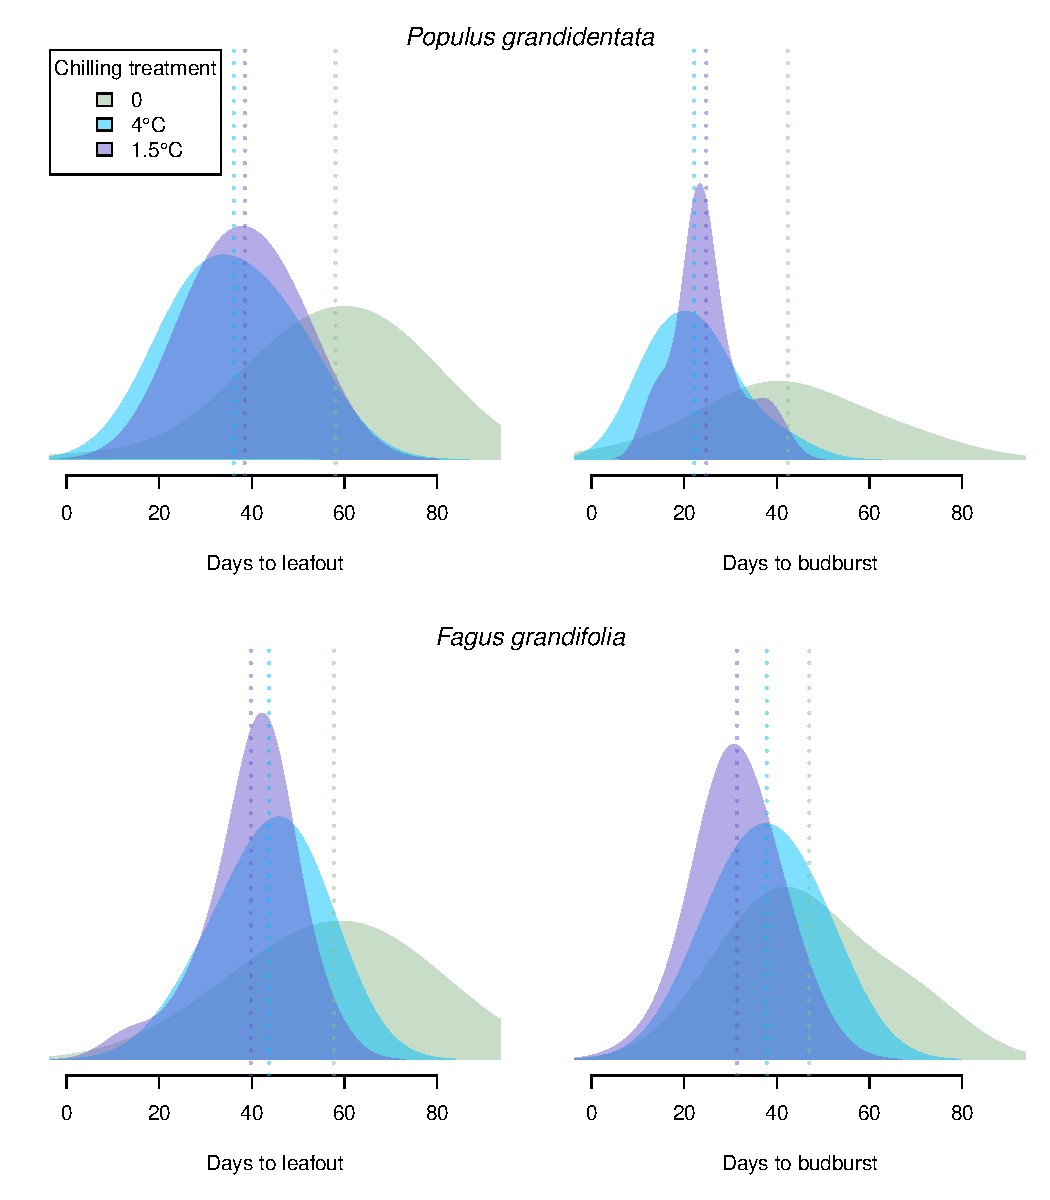
\includegraphics[scale=0.65]{Chillplot}
\end{center}

\subsection*{Species-specific responses}


Species traits partly explain variation in budburst and leafout. Plant with high nitrogen leaves, as well as high SLA (thinner, less dense) leaves, were significantly later in both budburst and leafout. Thus early leafout species tended to be tougher, less N-dense, and have higher carbon investments than later species. Greater wood density had inconsitent effects as a driver, with higher wood density driving later budburst but tending to drive earlier leafout.

Ring-porous species (Fraxinus sp., Lonicera, Myrica, and Quercus; lower values of Pore Anatomy variable) exhibited significantly later budburst and leafout compared to diffuse-porous species, in line with previous work on wood anatomy and freezing risk (Sperrry \& Sullivan 1991 Plant Phys).

Table 3. Summary of species-specific predictors of budburst day. Greater wood density, high specific leaf area (thinner/less dense leaves) and high leaf \% N resulted in later budburst date, while diffuse porous anatomy resulted in earlier budburst.

\FloatBarrier
\begin{table}[ht]
\centering
\begin{tabular}{rrrrrrr}
  \hline
 & est & se & stat & p & lwr & upr \\ 
  \hline
Intercept & 26.48 & 0.30 & 88.55 & 0.00 & 25.90 & 27.07 \\ 
  Wood density & 2.02 & 0.36 & 5.65 & 0.00 & 1.32 & 2.73 \\ 
  SLA & 2.18 & 0.30 & 7.21 & 0.00 & 1.59 & 2.78 \\ 
  \% N & 4.00 & 0.34 & 11.61 & 0.00 & 3.32 & 4.67 \\ 
  Pore Anatomy & -3.69 & 0.31 & -11.82 & 0.00 & -4.30 & -3.08 \\ 
   \hline
\end{tabular}
\end{table}
\FloatBarrier

Table 4. Summary of species-specific predictors of leafout day. Greater wood density (n.s.) and tendancy to be diffuse porous resulted in earlier leafout, while high specific leaf area (thinner/less dense leaves) and high leaf \% N resulted in later leafout.

\FloatBarrier
\begin{table}[ht]
\centering
\begin{tabular}{rrrrrrr}
  \hline
 & est & se & stat & p & lwr & upr \\ 
  \hline
 Intercept & 37.44 & 0.37 & 102.24 & 0.00 & 36.72 & 38.15 \\ 
  Wood density & -0.18 & 0.46 & -0.38 & 0.70 & -1.08 & 0.73 \\ 
  SLA & 1.83 & 0.37 & 4.95 & 0.00 & 1.11 & 2.56 \\ 
  \% N & 3.97 & 0.43 & 9.28 & 0.00 & 3.13 & 4.81 \\ 
Pore Anatomy & -0.89 & 0.38 & -2.36 & 0.02 & -1.63 & -0.15 \\ 
   \hline
\end{tabular}
\end{table}
\FloatBarrier

Table 5. Phylogenetic signal in timing of budburst and leafout and species specific traits. Pore anatomy (ring- versus diffuse-porous species) was highly clustered phylogenetically, but no other trait examined demonstrated significant phylogenetic signal. 

\FloatBarrier
\begin{table}[ht]
\centering
\begin{tabular}{rlrrr}
  \hline
 & Variable & K & PIC variance & PIC variance P \\ 
  \hline
1 & Budburst & 0.02 & 47.53 & 0.73 \\ 
  2 & Leafout & 0.03 & 38.47 & 0.58 \\ 
  3 & Wood Density & 0.25 & 0.04 & 0.06 \\ 
  4 & Pore anatomy & 1.38 & 0.01 & 0.00 \\ 
  5 & SLA & 0.15 & 240.79 & 0.19 \\ 
  6 & \% N & 0.19 & 0.01 & 0.12 \\ 
   \hline
\end{tabular}
\end{table}
\FloatBarrier

Figure 5. Summary of relationships between budburst day, leafout day, and plant functional traits.

\begin{center}
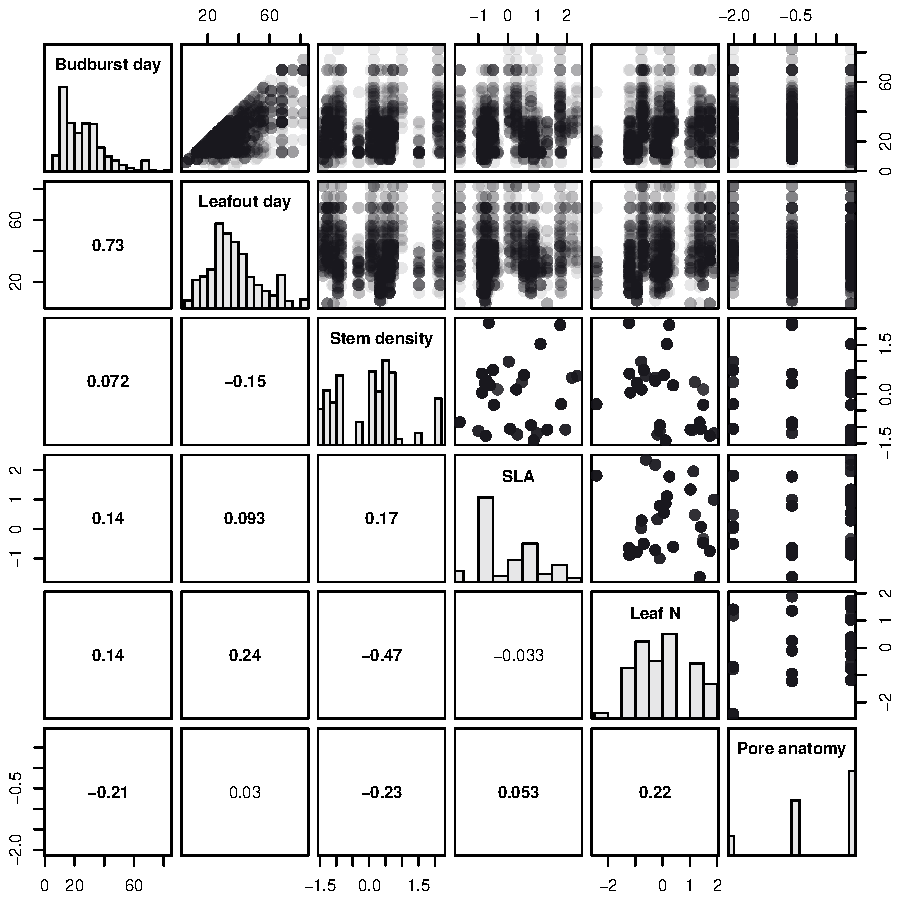
\includegraphics[scale=0.75]{traitpairs}
\end{center}

Figure 6. Individual-level variation for each population (latitude of origin) for each of the 28 species studied. Later-leafing out species were more consistent in their days to leafout across treatments, indicating greater phenotypic plasticity.

\begin{center}
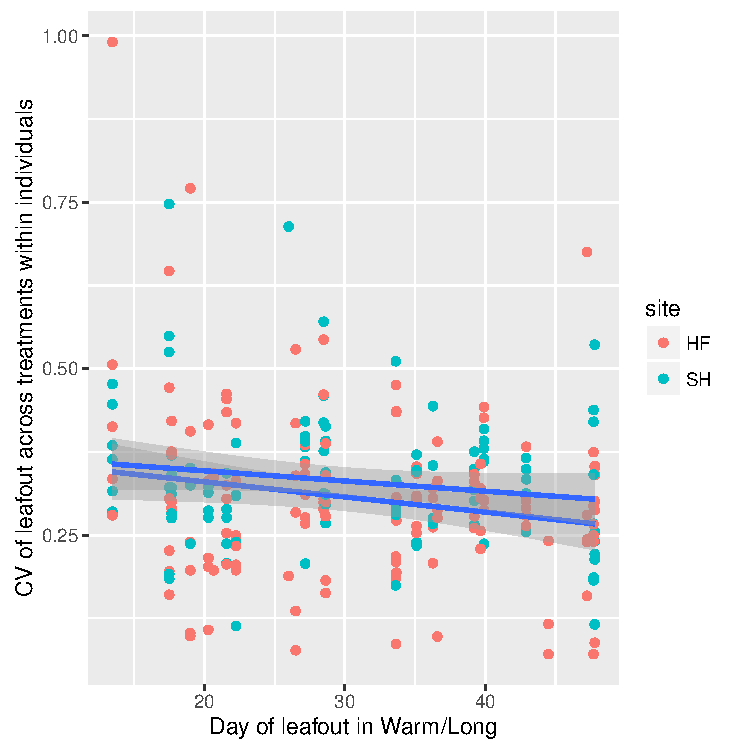
\includegraphics[scale=0.75]{indvar}
\end{center}

\subsection{Nonleafouts}

Separate analysis of samples which did not break bud or leafout. Across species, there was no overall predictive effect of temperature, photoperiod, chilling, or site on the propensity to fail to leaf out. 
Species ranged from complete leafout (Hamamelis) to only 50\% leafout (Fagus grandifolia, Acer saccharum) across all treatments. The percent of nonleafout s by site was similar, with 12.4\% of Harvard Forest and 9.5\% of St. Hippolyte samples failing to leaf out. Examining individual species,  there was an interaction of temperatuer by daylength for some species, with greater failure to leafout in cool, short conditions for Acer pensylvanicum  and Acer saccharum. Site effects were in consistent, with greater failure to leafout for cuttings from St. Hippolyte in Acer rubrum and Fagus grandifolia, and from Harvard Forest in Acer saccharum.

\section{Discussion}

\begin{itemize}

\item{Photoperiod sensitivity is common in northeastern woody plants; Phenological sensitivity to photoperiod and temperature are largely coordinated across species.}
\item{Under warming climates, shrubs and small trees are more opportunistic with novel climate conditions. Larger trees, being less sensitive to temperature cues, will be challenged. }
\item{Initial analysis shows little increase in risk-avoidance strategies for northern populations of these 28 species}
\item{Future work will integrate bud and wood anatomy and leaf functional traits to develop species-level predictions of northeastern forest phenological change under future climate conditions.}
\end{itemize}

\section{Supplemental Figures and Tables}

% Stan output for budburst day of year model

Supplemental Table 2. Stan output for analysis of budburst day by species and site. Parameters for site (a1 and a2) and species-level parameters for effects of warming (b\_warm), photoperiod (b\_photo), chilling (b\_chill), and the interaction of warming and photoperiod (b\_inter) shown.
\FloatBarrier
\begin{table}[ht]
\centering
\begin{tabular}{rrrrr}
  \hline
 & mean & se\_mean & sd & Rhat \\ 
  \hline
a[1] & 32.38 & 1.37 & 1.93 & 103.13 \\ 
  a[2] & 35.61 & 1.64 & 2.32 & 140.06 \\ 
  b\_warm[1] & 0.75 & 3.79 & 5.36 & 294.57 \\ 
  b\_warm[2] & 2.57 & 2.84 & 4.02 & 70.49 \\ 
  b\_warm[3] & 4.93 & 6.43 & 9.09 & 187.11 \\ 
  b\_warm[4] & -4.55 & 1.91 & 2.71 & 56.33 \\ 
  b\_warm[5] & -9.51 & 1.97 & 2.79 & 64.56 \\ 
  b\_warm[6] & 2.73 & 1.38 & 1.96 & 72.87 \\ 
  b\_warm[7] & -7.35 & 4.15 & 5.88 & 186.35 \\ 
  b\_warm[8] & 0.80 & 1.98 & 2.80 & 45.88 \\ 
  b\_warm[9] & -2.87 & 1.69 & 2.39 & 56.36 \\ 
  b\_warm[10] & 13.30 & 5.46 & 7.73 & 152.62 \\ 
  b\_warm[11] & -5.30 & 1.96 & 2.77 & 61.93 \\ 
  b\_warm[12] & -3.79 & 7.72 & 10.92 & 133.20 \\ 
  b\_warm[13] & -0.25 & 1.62 & 2.30 & 35.34 \\ 
  b\_warm[14] & -9.71 & 3.64 & 5.15 & 114.41 \\ 
  b\_warm[15] & -10.45 & 4.54 & 6.43 & 116.01 \\ 
  b\_warm[16] & -19.76 & 2.18 & 3.09 & 44.55 \\ 
  b\_warm[17] & -5.71 & 2.87 & 4.07 & 75.30 \\ 
  b\_warm[18] & 7.76 & 2.15 & 3.04 & 53.46 \\ 
  b\_warm[19] & -0.03 & 3.63 & 5.14 & 63.91 \\ 
  b\_warm[20] & 18.03 & 9.35 & 13.23 & 277.82 \\ 
  b\_warm[21] & 1.32 & 2.36 & 3.35 & 48.05 \\ 
  b\_warm[22] & 10.85 & 3.48 & 4.92 & 181.06 \\ 
  b\_warm[23] & 5.72 & 3.09 & 4.37 & 122.41 \\ 
  b\_warm[24] & 2.05 & 4.08 & 5.77 & 37.52 \\ 
  b\_warm[25] & -7.87 & 4.39 & 6.20 & 219.91 \\ 
  b\_warm[26] & -8.71 & 4.88 & 6.90 & 279.74 \\ 
  b\_warm[27] & -5.02 & 1.06 & 1.51 & 38.68 \\ 
  b\_warm[28] & -1.65 & 0.65 & 0.92 & 25.51 \\ 
  b\_photo[1] & -3.59 & 3.84 & 5.43 & 122.27 \\ 
  b\_photo[2] & -2.86 & 3.44 & 4.87 & 98.34 \\ 
  b\_photo[3] & 7.54 & 4.86 & 6.88 & 126.61 \\ 
  b\_photo[4] & 2.31 & 1.90 & 2.69 & 48.66 \\ 
  b\_photo[5] & -8.84 & 4.17 & 5.90 & 265.88 \\ 
  b\_photo[6] & -0.43 & 1.31 & 1.86 & 51.85 \\ 
  b\_photo[7] & -4.81 & 5.47 & 7.74 & 110.56 \\ 
  b\_photo[8] & 0.80 & 1.15 & 1.63 & 106.36 \\ 
  b\_photo[9] & -2.56 & 0.81 & 1.15 & 26.99 \\ 
  b\_photo[10] & 4.15 & 4.80 & 6.80 & 45.34 \\ 
  b\_photo[11] & 0.76 & 2.81 & 3.98 & 61.24 \\ 
  b\_photo[12] & -4.51 & 6.71 & 9.49 & 308.92 \\ 
  b\_photo[13] & -2.41 & 1.57 & 2.22 & 64.71 \\ 
  b\_photo[14] & -3.14 & 3.58 & 5.07 & 144.29 \\ 
  b\_photo[15] & -3.72 & 5.60 & 7.92 & 266.71 \\ 
  b\_photo[16] & -9.56 & 4.90 & 6.93 & 186.26 \\ 
  b\_photo[17] & -3.43 & 2.48 & 3.50 & 232.59 \\ 
  b\_photo[18] & 12.26 & 3.31 & 4.69 & 191.36 \\ 
  b\_photo[19] & -0.47 & 2.58 & 3.65 & 77.23 \\ 
  b\_photo[20] & 3.82 & 4.14 & 5.86 & 148.48 \\ 
  b\_photo[21] & 2.52 & 3.83 & 5.43 & 65.07 \\ 
  b\_photo[22] & 25.23 & 3.78 & 5.35 & 186.10 \\ 
  b\_photo[23] & 17.12 & 6.78 & 9.60 & 66.23 \\ 
  b\_photo[24] & 16.76 & 4.95 & 7.00 & 89.83 \\ 
  b\_photo[25] & -9.07 & 7.10 & 10.04 & 268.49 \\ 
  b\_photo[26] & -5.37 & 4.78 & 6.76 & 259.53 \\ 
  b\_photo[27] & -7.42 & 1.13 & 1.60 & 75.26 \\ 
  b\_photo[28] & 4.17 & 1.83 & 2.60 & 64.39 \\ 
  b\_chill[1] & -2.12 & 46.50 & 65.79 & 764.55 \\ 
  b\_chill[2] & 23.74 & 25.72 & 36.40 & 368.58 \\ 
  b\_chill[3] & -0.78 & 5.16 & 7.31 & 69.06 \\ 
  b\_chill[4] & 22.95 & 13.56 & 19.20 & 81.07 \\ 
  b\_chill[5] & 14.22 & 23.51 & 33.26 & 1182.72 \\ 
  b\_chill[6] & 3.44 & 9.13 & 12.92 & 169.80 \\ 
  b\_chill[7] & -19.86 & 15.11 & 21.38 & 396.34 \\ 
  b\_chill[8] & -3.30 & 24.59 & 34.80 & 456.30 \\ 
  b\_chill[9] & 1.44 & 10.58 & 14.97 & 324.73 \\ 
  b\_chill[10] & 1.33 & 24.85 & 35.17 & 695.53 \\ 
  b\_chill[11] & -13.16 & 20.30 & 28.73 & 327.09 \\ 
  b\_chill[12] & 19.58 & 19.51 & 27.60 & 1020.54 \\ 
  b\_chill[13] & -12.43 & 9.00 & 12.74 & 390.82 \\ 
  b\_chill[14] & -8.92 & 21.76 & 30.78 & 593.98 \\ 
  b\_chill[15] & -10.95 & 17.72 & 25.07 & 292.72 \\ 
  b\_chill[16] & -35.42 & 10.72 & 15.17 & 104.60 \\ 
  b\_chill[17] & 1.66 & 25.01 & 35.38 & 960.18 \\ 
  b\_chill[18] & 4.61 & 10.70 & 15.13 & 269.74 \\ 
  b\_chill[19] & -24.14 & 12.50 & 17.69 & 1075.04 \\ 
  b\_chill[20] & 12.00 & 22.91 & 32.42 & 671.13 \\ 
  b\_chill[21] & 11.42 & 8.63 & 12.21 & 295.01 \\ 
  b\_chill[22] & 11.89 & 11.67 & 16.51 & 236.71 \\ 
  b\_chill[23] & 0.25 & 29.01 & 41.05 & 748.93 \\ 
  b\_chill[24] & 16.26 & 19.92 & 28.19 & 574.01 \\ 
  b\_chill[25] & -0.65 & 17.45 & 24.70 & 526.53 \\ 
  b\_chill[26] & 4.09 & 25.33 & 35.84 & 699.99 \\ 
  b\_chill[27] & -1.16 & 9.56 & 13.52 & 363.96 \\ 
  b\_chill[28] & -5.93 & 22.85 & 32.33 & 208.79 \\ 
  b\_inter[1] & -0.87 & 2.50 & 3.54 & 89.77 \\ 
  b\_inter[2] & -2.10 & 2.22 & 3.14 & 106.12 \\ 
  b\_inter[3] & -9.55 & 3.36 & 4.76 & 52.79 \\ 
  b\_inter[4] & -4.44 & 1.23 & 1.74 & 24.41 \\ 
  b\_inter[5] & 5.96 & 1.87 & 2.64 & 65.95 \\ 
  b\_inter[6] & -2.96 & 0.68 & 0.97 & 45.51 \\ 
  b\_inter[7] & 2.07 & 3.32 & 4.70 & 82.21 \\ 
  b\_inter[8] & -2.19 & 0.74 & 1.05 & 35.32 \\ 
  b\_inter[9] & -2.22 & 0.63 & 0.90 & 34.10 \\ 
  b\_inter[10] & -11.58 & 2.88 & 4.08 & 194.12 \\ 
  b\_inter[11] & -3.04 & 1.63 & 2.30 & 104.61 \\ 
  b\_inter[12] & -3.92 & 4.02 & 5.69 & 50.95 \\ 
  b\_inter[13] & -1.03 & 0.60 & 0.85 & 39.84 \\ 
  b\_inter[14] & 0.63 & 2.36 & 3.34 & 57.30 \\ 
  b\_inter[15] & 3.02 & 3.73 & 5.27 & 172.59 \\ 
  b\_inter[16] & 7.04 & 2.03 & 2.87 & 106.50 \\ 
  b\_inter[17] & -0.43 & 1.99 & 2.82 & 104.62 \\ 
  b\_inter[18] & -10.99 & 2.59 & 3.67 & 90.36 \\ 
  b\_inter[19] & -0.98 & 1.48 & 2.09 & 80.92 \\ 
  b\_inter[20] & -10.31 & 5.75 & 8.14 & 225.61 \\ 
  b\_inter[21] & -5.39 & 2.05 & 2.91 & 151.35 \\ 
  b\_inter[22] & -19.36 & 3.06 & 4.32 & 89.80 \\ 
  b\_inter[23] & -12.88 & 2.94 & 4.16 & 138.45 \\ 
  b\_inter[24] & -9.65 & 3.44 & 4.87 & 40.28 \\ 
  b\_inter[25] & 3.44 & 4.64 & 6.57 & 237.49 \\ 
  b\_inter[26] & 1.70 & 3.00 & 4.24 & 224.67 \\ 
  b\_inter[27] & 1.34 & 0.84 & 1.19 & 50.72 \\ 
  b\_inter[28] & -4.51 & 1.20 & 1.70 & 57.34 \\ 
   \hline
\end{tabular}
\end{table}
\FloatBarrier

Supplemental Table 2. Stan output for analysis of leafout day by species and site. Parameters for site (a1 and a2) and species-level parameters for effects of warming (b\_warm), photoperiod (b\_photo), chilling (b\_chill), and the interaction of warming and photoperiod (b\_inter) shown.
\FloatBarrier
\begin{table}[ht]
\centering
\begin{tabular}{rrrrr}
  \hline
 & mean & se\_mean & sd & Rhat \\ 
  \hline
a[1] & 79.67 & 3.54 & 5.01 & 80.47 \\ 
  a[2] & 75.92 & 4.09 & 5.79 & 50.31 \\ 
  b\_warm[1] & -13.01 & 3.13 & 4.43 & 83.70 \\ 
  b\_warm[2] & -12.04 & 2.28 & 3.23 & 47.46 \\ 
  b\_warm[3] & -9.67 & 6.51 & 9.21 & 272.99 \\ 
  b\_warm[4] & -10.94 & 4.96 & 7.02 & 70.54 \\ 
  b\_warm[5] & -18.92 & 3.21 & 4.55 & 75.95 \\ 
  b\_warm[6] & -17.20 & 1.36 & 1.94 & 22.69 \\ 
  b\_warm[7] & -25.56 & 2.34 & 3.31 & 51.82 \\ 
  b\_warm[8] & -15.72 & 1.55 & 2.20 & 12.09 \\ 
  b\_warm[9] & -16.80 & 2.55 & 3.61 & 44.28 \\ 
  b\_warm[10] & -6.37 & 1.88 & 2.66 & 52.01 \\ 
  b\_warm[11] & -15.89 & 2.34 & 3.32 & 33.57 \\ 
  b\_warm[12] & -21.45 & 4.85 & 6.87 & 93.58 \\ 
  b\_warm[13] & -17.37 & 2.29 & 3.24 & 64.42 \\ 
  b\_warm[14] & -12.28 & 4.74 & 6.71 & 55.84 \\ 
  b\_warm[15] & -26.94 & 3.87 & 5.48 & 67.36 \\ 
  b\_warm[16] & -25.43 & 6.33 & 8.96 & 52.14 \\ 
  b\_warm[17] & -12.47 & 8.87 & 12.55 & 111.97 \\ 
  b\_warm[18] & -7.27 & 2.43 & 3.45 & 15.35 \\ 
  b\_warm[19] & -23.88 & 2.61 & 3.70 & 41.07 \\ 
  b\_warm[20] & -15.17 & 4.38 & 6.20 & 36.90 \\ 
  b\_warm[21] & -12.50 & 2.41 & 3.42 & 69.20 \\ 
  b\_warm[22] & -10.81 & 4.19 & 5.93 & 96.76 \\ 
  b\_warm[23] & -26.68 & 1.96 & 2.78 & 23.99 \\ 
  b\_warm[24] & -4.53 & 6.43 & 9.11 & 25.95 \\ 
  b\_warm[25] & -26.83 & 3.01 & 4.27 & 20.73 \\ 
  b\_warm[26] & -24.08 & 1.77 & 2.51 & 20.89 \\ 
  b\_warm[27] & -14.53 & 4.10 & 5.81 & 44.59 \\ 
  b\_warm[28] & -14.79 & 2.40 & 3.39 & 34.55 \\ 
  b\_photo[1] & -10.18 & 4.14 & 5.86 & 255.01 \\ 
  b\_photo[2] & -12.79 & 2.31 & 3.28 & 39.01 \\ 
  b\_photo[3] & -5.01 & 7.58 & 10.72 & 135.01 \\ 
  b\_photo[4] & -5.35 & 2.86 & 4.05 & 14.68 \\ 
  b\_photo[5] & -13.99 & 3.00 & 4.24 & 67.33 \\ 
  b\_photo[6] & -17.25 & 1.07 & 1.51 & 31.35 \\ 
  b\_photo[7] & -14.94 & 4.47 & 6.33 & 50.05 \\ 
  b\_photo[8] & -12.43 & 1.23 & 1.76 & 15.83 \\ 
  b\_photo[9] & -13.19 & 1.32 & 1.87 & 13.08 \\ 
  b\_photo[10] & -4.50 & 2.69 & 3.81 & 33.82 \\ 
  b\_photo[11] & -7.60 & 0.58 & 0.90 & 3.07 \\ 
  b\_photo[12] & -16.02 & 5.20 & 7.36 & 46.66 \\ 
  b\_photo[13] & -19.29 & 2.60 & 3.68 & 30.18 \\ 
  b\_photo[14] & 3.71 & 9.79 & 13.87 & 38.29 \\ 
  b\_photo[15] & -23.34 & 1.13 & 1.66 & 4.38 \\ 
  b\_photo[16] & -4.16 & 2.56 & 3.63 & 69.87 \\ 
  b\_photo[17] & -6.95 & 5.95 & 8.42 & 68.25 \\ 
  b\_photo[18] & -0.10 & 2.26 & 3.20 & 18.61 \\ 
  b\_photo[19] & -14.18 & 2.99 & 4.23 & 20.45 \\ 
  b\_photo[20] & -9.56 & 5.52 & 7.81 & 91.19 \\ 
  b\_photo[21] & -9.08 & 1.07 & 1.52 & 14.24 \\ 
  b\_photo[22] & -0.47 & 4.45 & 6.30 & 52.00 \\ 
  b\_photo[23] & -10.65 & 2.86 & 4.05 & 28.28 \\ 
  b\_photo[24] & 3.35 & 6.49 & 9.19 & 77.87 \\ 
  b\_photo[25] & -22.49 & 4.28 & 6.07 & 21.88 \\ 
  b\_photo[26] & -17.47 & 2.68 & 3.80 & 28.81 \\ 
  b\_photo[27] & -14.63 & 4.32 & 6.12 & 124.02 \\ 
  b\_photo[28] & -15.53 & 1.24 & 1.76 & 12.55 \\ 
  b\_chill[1] & 20.04 & 14.70 & 20.79 & 365.72 \\ 
  b\_chill[2] & 28.87 & 36.05 & 51.01 & 330.04 \\ 
  b\_chill[3] & 11.69 & 8.49 & 12.02 & 57.22 \\ 
  b\_chill[4] & -10.85 & 32.06 & 45.36 & 346.65 \\ 
  b\_chill[5] & -15.95 & 22.38 & 31.67 & 312.74 \\ 
  b\_chill[6] & 1.88 & 39.14 & 55.38 & 173.76 \\ 
  b\_chill[7] & 6.23 & 36.44 & 51.56 & 228.96 \\ 
  b\_chill[8] & 16.05 & 23.29 & 32.95 & 114.18 \\ 
  b\_chill[9] & -25.31 & 13.58 & 19.22 & 77.29 \\ 
  b\_chill[10] & 50.31 & 12.32 & 17.43 & 282.36 \\ 
  b\_chill[11] & 1.96 & 24.67 & 34.90 & 249.30 \\ 
  b\_chill[12] & 2.98 & 28.50 & 40.33 & 222.23 \\ 
  b\_chill[13] & 8.77 & 14.65 & 20.74 & 29.31 \\ 
  b\_chill[14] & 7.45 & 29.30 & 41.46 & 99.44 \\ 
  b\_chill[15] & 4.84 & 9.97 & 14.11 & 77.31 \\ 
  b\_chill[16] & -2.29 & 12.31 & 17.42 & 171.98 \\ 
  b\_chill[17] & -30.48 & 13.11 & 18.55 & 256.72 \\ 
  b\_chill[18] & 2.80 & 16.70 & 23.62 & 213.24 \\ 
  b\_chill[19] & -10.38 & 12.83 & 18.15 & 184.26 \\ 
  b\_chill[20] & 3.32 & 17.66 & 24.99 & 143.07 \\ 
  b\_chill[21] & 0.47 & 10.67 & 15.10 & 278.33 \\ 
  b\_chill[22] & 24.89 & 12.24 & 17.32 & 146.39 \\ 
  b\_chill[23] & 45.45 & 18.08 & 25.59 & 193.32 \\ 
  b\_chill[24] & 8.55 & 20.15 & 28.52 & 222.89 \\ 
  b\_chill[25] & 17.49 & 26.35 & 37.28 & 263.84 \\ 
  b\_chill[26] & 2.13 & 14.56 & 20.60 & 169.64 \\ 
  b\_chill[27] & 12.85 & 13.98 & 19.79 & 67.02 \\ 
  b\_chill[28] & -10.08 & 26.88 & 38.03 & 404.36 \\ 
  b\_inter[1] & -0.75 & 2.06 & 2.92 & 115.33 \\ 
  b\_inter[2] & 1.74 & 1.14 & 1.62 & 16.31 \\ 
  b\_inter[3] & -3.27 & 3.51 & 4.96 & 69.18 \\ 
  b\_inter[4] & -3.01 & 1.85 & 2.62 & 18.56 \\ 
  b\_inter[5] & 4.53 & 2.29 & 3.24 & 33.08 \\ 
  b\_inter[6] & 5.29 & 0.34 & 0.48 & 19.17 \\ 
  b\_inter[7] & 3.20 & 2.12 & 3.00 & 17.44 \\ 
  b\_inter[8] & 4.16 & 1.15 & 1.63 & 17.35 \\ 
  b\_inter[9] & 0.08 & 1.14 & 1.63 & 17.82 \\ 
  b\_inter[10] & -3.78 & 1.91 & 2.70 & 80.43 \\ 
  b\_inter[11] & -1.76 & 1.14 & 1.62 & 19.58 \\ 
  b\_inter[12] & 2.81 & 4.23 & 5.99 & 38.75 \\ 
  b\_inter[13] & 5.21 & 1.73 & 2.45 & 42.57 \\ 
  b\_inter[14] & -14.17 & 4.70 & 6.65 & 58.21 \\ 
  b\_inter[15] & 9.68 & 1.15 & 1.63 & 22.28 \\ 
  b\_inter[16] & -0.10 & 3.98 & 5.63 & 39.98 \\ 
  b\_inter[17] & -3.77 & 5.65 & 7.99 & 71.81 \\ 
  b\_inter[18] & -6.33 & 1.40 & 1.99 & 21.87 \\ 
  b\_inter[19] & 6.09 & 1.49 & 2.11 & 18.16 \\ 
  b\_inter[20] & -0.28 & 2.79 & 3.95 & 39.19 \\ 
  b\_inter[21] & 0.31 & 0.90 & 1.28 & 10.20 \\ 
  b\_inter[22] & -4.24 & 4.26 & 6.03 & 40.89 \\ 
  b\_inter[23] & 1.51 & 1.78 & 2.52 & 32.01 \\ 
  b\_inter[24] & -9.29 & 6.57 & 9.29 & 132.43 \\ 
  b\_inter[25] & 11.61 & 2.47 & 3.49 & 24.12 \\ 
  b\_inter[26] & 8.52 & 1.31 & 1.85 & 35.04 \\ 
  b\_inter[27] & 6.37 & 2.56 & 3.62 & 144.12 \\ 
  b\_inter[28] & 5.00 & 1.26 & 1.79 & 21.09 \\ 
   \hline
\end{tabular}
\end{table}
\FloatBarrier

\end{document}